\documentclass[11pt,a4paper]{article}

\usepackage[utf8]{inputenc}
\usepackage[margin=2.5cm]{geometry}
\usepackage{amsmath,amssymb,amsfonts}
\usepackage{mathtools}
\usepackage{siunitx}
\usepackage{threeparttable}
\usepackage{centernot}
\usepackage{multirow}
\usepackage{booktabs}
\usepackage{tabularx}
\usepackage{graphicx}
\usepackage{float}
\usepackage{url}
\usepackage{hyperref}
\hypersetup{hidelinks,hypertexnames=false}
\usepackage{cite}
\usepackage{caption}
\usepackage{microtype}
\usepackage{placeins}
\usepackage{needspace}
\usepackage{authblk}

% Pseudo-code packages
\usepackage{algorithm}
\usepackage{algpseudocode}

% Source-code listings
\usepackage{listings}

\newcommand{\cmark}{\checkmark}
\newcommand{\xmark}{\times}
\newcommand{\etal}{\emph{et al.}}

% Publisher-neutral macros matching preprints requirements
\newcommand{\Title}[1]{\title{\textbf{\Large #1}}}
\newcommand{\authorcontributions}[1]{\par\medskip\noindent\textbf{Author Contributions: }#1}
\newcommand{\funding}[1]{\par\smallskip\noindent\textbf{Funding: }#1}
\newcommand{\institutionalreview}[1]{\par\smallskip\noindent\textbf{Institutional Review Board Statement: }#1}
\newcommand{\informedconsent}[1]{\par\smallskip\noindent\textbf{Informed Consent Statement: }#1}
\newcommand{\dataavailability}[1]{\par\smallskip\noindent\textbf{Data Availability Statement: }#1}
\newcommand{\conflictsofinterest}[1]{\par\smallskip\noindent\textbf{Conflicts of Interest: }#1}

\title{\textbf{\Large Scalability-Aware Benchmarking of Graph Anomaly Detection on Financial and Cyber Networks: Evaluated Population, Alert Budgets, and the Exact Limits of Decoupled GNNs}}

\author[1]{Seong-Su Park\thanks{ORCID: \url{https://orcid.org/0009-0008-4056-3875}}}
\author[2]{Ki-Hyung Kim\thanks{Corresponding author: \texttt{kkim86@ajou.ac.kr}; Tel.: +82-31-219-2433; ORCID: \url{https://orcid.org/0000-0002-2321-4475}}}

\affil[1]{\small Department of Computer Engineering, Ajou University, Suwon 16499, Republic of Korea; \texttt{parky@ajou.ac.kr}}
\affil[2]{\small Department of Cyber Security, Ajou University, Suwon 16499, Republic of Korea; \texttt{kkim86@ajou.ac.kr}}

\date{\today}

\begin{document}
\maketitle

\begin{abstract}
Graph anomaly detection (GAD) is increasingly adopted for financial fraud mitigation and cyber intrusion defense. However, real-world deployment faces severe obstacles: out-of-memory (OOM) failures on massive graphs are often obscured by selective reporting, severe class imbalance invalidates plain ROC-AUC rankings, and unsupervised reconstruction objectives can exhibit empirical rankings that invert expected anomaly ordering on complex transaction graphs. To establish a rigorous, application-oriented benchmark, we evaluate seven functioning primary detectors (DOMINANT, AnomalyDAE, CoLA, GADNR, OCGNN, DLG-Base, and DLG-Aug) across 13 primary graph benchmarks (five native financial, eight synthetic injected) and one external enterprise cybersecurity network (LANL-RedTeam) over five random seeds (455 total runs). We enforce a strict support-aware contract: 84 of 91 primary model--dataset pairs are successfully completed, while unsupported cells are reported transparently rather than silently imputed. 

Our empirical results reveal critical domain-dependent behaviors. While Decoupled Local-to-Global augmentation (DLG-Aug) improves average precision (AP) over the DLG-Base reference on the Elliptic transaction network by $+0.0350$ (0.1037 vs.\ 0.0687), it suffers an AP degradation of $-0.0656$ on the large Reddit-Syn graph (0.3388 vs.\ 0.4044) and exhibits negative delta on LANL-RedTeam. On blockchain token-transfer networks, at least one established comparator exceeds DLG-Aug in mean AP on each of the three blockchain datasets (Ethereum: OCGNN $0.4996$ vs.\ Aug $0.4359$; BSC: AnomalyDAE $0.3609$ vs.\ Aug $0.3411$; Polygon: AnomalyDAE $0.1878$ vs.\ Aug $0.0731$). Furthermore, several unsupervised reconstruction models obtain below-random ROC-AUC values ($<0.50$) on Elliptic under standard detector orientation. While topological degree heterogeneity and licit hub reconstruction patterns represent plausible explanatory hypotheses, historical node-level score arrays were not archived by the benchmark runner, precluding causal verification; we report authentic empirical rankings without post-hoc sign inversion. Finally, we provide closed-form exact Gram decoders that eliminate dense $O(N^2)$ memory allocation and present a practical decision matrix connecting alert budgets (top-1\% and top-5\%) to operational detector selection.
\end{abstract}

\noindent{\small\textbf{Keywords: }graph anomaly detection; graph neural networks; financial fraud detection; alert budget; exact sparse reconstruction; reproducible benchmarking; local-to-global learning}\par

\section{Introduction}
\label{sec:introduction}
Graph anomaly detection (GAD) has emerged as a cornerstone of modern machine learning for financial fraud investigation, blockchain anti-money laundering (AML), and enterprise cybersecurity monitoring \cite{ma2023survey,qiao2025survey,dilini2026comprehensive}. By modeling transactions, contracts, and authentication events as interconnected graphs $G=(V, E, X)$, graph neural networks (GNNs) can capture subtle topological irregularities and feature discrepancies that evade tabular screening.

However, moving GAD from idealized academic benchmarks to operational deployment reveals fundamental challenges that conventional evaluation protocols frequently obscure:
\begin{enumerate}
    \item \textbf{Failure-Blind Reporting and Hardware Infeasibility:} Standard leaderboards often omit unsupported cells when models suffer out-of-memory (OOM) crashes or runtime timeouts on web-scale or multi-million-node graphs, or they quietly replace the full-graph objective with localized neighborhood sampling without verifying whether score semantics are preserved.
    \item \textbf{Imbalance Disconnect and Below-Random Behavior:} In real-world financial fraud, anomaly prevalence is frequently below 2\% or 0.5\%. In these extreme regimes, high area under the ROC curve (ROC-AUC) can be misleading. More critically, unsupervised reconstruction models often exhibit empirical ROC-AUC scores falling well below the 0.50 random baseline on financial transaction networks such as Elliptic under standard score conventions. While topological characteristics such as high-degree licit transaction hubs have been hypothesized to incur disproportionate reconstruction errors, the absence of archived per-node score arrays precludes causal attribution; we document this below-random behavior as an authentic empirical finding without heuristic sign inversion.
    \item \textbf{Alert-Budget Constraints:} Security operations centers (SOCs) and fraud investigation teams cannot inspect thousands of suspicious accounts; they operate under strict investigative triage budgets (e.g., auditing the top-1\% or top-5\% flagged alerts). Ranking metrics alone do not tell practitioners whether a detector provides actionable precision at the head of the flagged list.
    \item \textbf{Conditional Utility of Architecture Augmentation:} Pretraining local graph representations and fusing them with global message passing (e.g., Decoupled Local-to-Global architectures, DLG \cite{park2026dlg}) has demonstrated strong performance in specific cryptocurrency domains, but its comparative utility across diverse topologies remains unverified under frozen, reproducible protocols.
\end{enumerate}

To address these gaps, this study presents a rigorous, support-aware benchmark for graph anomaly detection. We freeze seven representative detector configurations across 13 primary graph datasets and one external cybersecurity dataset, executing five random seeds per combination. Rather than claiming universal superiority for any single model, our benchmark contributes:
\begin{enumerate}
    \item \textbf{A Support-Aware Evaluation Protocol:} We explicitly distinguish between successful execution (`SUPPORTED\_EXACT') and hardware exhaustion (OOM), evaluating exactly 84 of 91 primary pairs ($420$ successful primary runs plus $35$ external LANL runs) without heuristic score imputation.
    \item \textbf{Audited Predictive Quality vs.\ Evaluation Prevalence and Alert Budgets:} We pair Average Precision (AP) with explicit evaluation prevalence references and evaluate triage precision and recall at fixed 1\% and 5\% alert budgets across financial and cyber graphs.
    \item \textbf{Rigorous Diagnosis of Below-Random Inversion:} We conduct an in-depth score, label, and mask audit of Elliptic and DGraphFin, demonstrating that below-0.50 ROC-AUC values reflect authentic empirical behavior under standard detector orientation rather than software defects, while exploring informed topological hypotheses.
    \item \textbf{Exact Closed-Form Decoupling Without Dense Materialization:} We mathematically derive and qualify closed-form Gram-matrix reconstructions that eliminate $N \times N$ dense adjacency storage, providing exact mathematical equivalence to dense loss evaluations for unsquashed dot-product decoders.
    \item \textbf{Application-Facing Decision Matrix:} We synthesize our findings into an actionable practitioner decision guide that maps graph density, feature availability, and alert budgets to optimal detector selection.
\end{enumerate}

\section{Related Work}
\label{sec:related}

\subsection{Unsupervised Graph Anomaly Detection}
Unsupervised GAD algorithms identify structural and contextual outliers without requiring ground-truth anomaly labels during training. DOMINANT \cite{ding2019deep} pioneered graph autoencoders by jointly minimizing attribute reconstruction error and dense adjacency reconstruction loss. AnomalyDAE \cite{fan2020anomalydae} employs dual autoencoders with cross-modal attention between structure and features. Contrastive methods such as CoLA \cite{liu2022cola} and CONAD \cite{xu2022conad} train local-to-subgraph mutual information estimators, scoring nodes by contrastive disagreement. One-class models such as OCGNN \cite{wang2021ocgnn} optimize a hypersphere enclosing normal representations, while GADNR \cite{roy2024gadnr} reconstructs neighborhood feature distributions via Gaussian mixture modeling. 

Benchmark libraries such as PyGOD \cite{liu2024pygod} and BOND \cite{liu2022bond} have standardized implementations on small and medium benchmarks. Recent investigations, such as GAD-in-the-Wild \cite{zhou2026wild}, have highlighted performance drops under realistic attribute corruption and low class prevalence. In cybersecurity, Dilini \etal\ \cite{dilini2026comprehensive} comprehensively reviewed graph-based anomaly detection methods for network intrusion detection, demonstrating that real-world authentication and flow graphs require specialized topological modeling. Our work builds upon this foundation by establishing hardware-aware execution boundaries and providing closed-form exact loss formulations for full-graph training.

\subsection{Imbalance-Aware Fraud Learning and Signed Networks}
Financial transaction graphs are characterized by extreme class skew and heterophily. Semi-supervised and supervised approaches such as PC-GNN \cite{liu2021pcgnn}, GraphSMOTE \cite{zhao2021graphsmote}, and Dual-Augment GNN \cite{li2022dualaugment} resample fraud distributions or penalize minority-class misclassification. In signed transaction networks, edge weights denote trust or distrust, as formalized by Kumar \etal\ \cite{kumar2016edge} in Bitcoin trust networks. For smart contract platforms, Jiang and Tsai \cite{jiang2025mvcg} proposed MVCG-SPS, a multi-view contrastive graph neural network for smart Ponzi scheme detection on Ethereum, demonstrating the effectiveness of decoupled relational perspectives. Because supervised fraud detectors require verified labels that are rarely available in early-stage forensics, this benchmark focuses primarily on unsupervised detectors, but incorporates alert-budget precision and recall to reflect practical operational requirements.

\subsection{Scalable Graph Learning and Sampling Limits}
To overcome the $O(N^2)$ memory bottleneck of dense adjacency matrices and full-graph convolutions, large-scale GNN frameworks employ neighborhood sampling (GraphSAGE \cite{hamilton2017graphsage}), layer sampling (FastGCN \cite{chen2018fastgcn}, LADIES \cite{zou2019ladies}), or graph partitioning (Cluster-GCN \cite{chiang2019clustergcn}, GraphSAINT \cite{zeng2020graphsaint}). While effective for node classification, sampling alters the empirical structural objective and can introduce variance that distorts reconstruction-based anomaly scores. Our approach instead retains the exact full-graph objective while leveraging algebraic reformulations to achieve scalable execution without sampling approximations.

\subsection{Benchmark Methodology and Evaluation Rigor}
Graph model rankings often exhibit strong sensitivity to split generation, hyperparameter choices, and random seeds \cite{shchur2018pitfalls,errica2020fair}. OGB \cite{hu2020ogb} and controlled benchmarking efforts \cite{dwivedi2023benchmarking} have emphasized the necessity of frozen data splits and transparent failure reporting. Crucially, Heidrich \etal\ \cite{heidrich2026systematic} established a systematic evaluation method for graph-derived signals, highlighting that multi-seed statistical significance and explicit dataset provenance are paramount when assessing model utility. Our protocol adheres to these principles by executing identical seed splits across all models, reporting non-parametric within-block permutation statistics, and leaving unsupported cells unscored.

\section{Decoupled GNNs and Exact Gram Sparse Decoders}
\label{sec:models}

\subsection{Evaluated Detector Architectures}
We evaluate seven functioning anomaly detector configurations spanning autoencoder, contrastive, one-class, and decoupled architectural families:
\begin{enumerate}
    \item \textbf{DOMINANT} \cite{ding2019deep}: GCN autoencoder reconstructing node attributes $X$ and dense adjacency $A$.
    \item \textbf{AnomalyDAE} \cite{fan2020anomalydae}: Dual autoencoder decoupling feature and structural embeddings via cross-modal attention.
    \item \textbf{CoLA} \cite{liu2022cola}: Contrastive self-supervised model evaluating local sub-graph agreement.
    \item \textbf{GADNR} \cite{roy2024gadnr}: Neighborhood distribution reconstruction with Gaussian mixture modeling.
    \item \textbf{OCGNN} \cite{wang2021ocgnn}: One-class classification optimizing a hypersphere enclosing normal representations.
    \item \textbf{DLG-Base} \cite{park2026dlg}: Standard GCN autoencoder employing exact sparse Gram loss evaluation.
    \item \textbf{DLG-Aug} \cite{park2026dlg}: Decoupled Local-to-Global model combining local ego-net pretraining with global propagation.
\end{enumerate}

\subsection{Decoupled Local-to-Global Architecture}
The overall workflow of the Decoupled Local-to-Global (DLG) architecture is illustrated in Figure~\ref{fig:dlg_architecture}.

\begin{figure}[htbp]
\centering
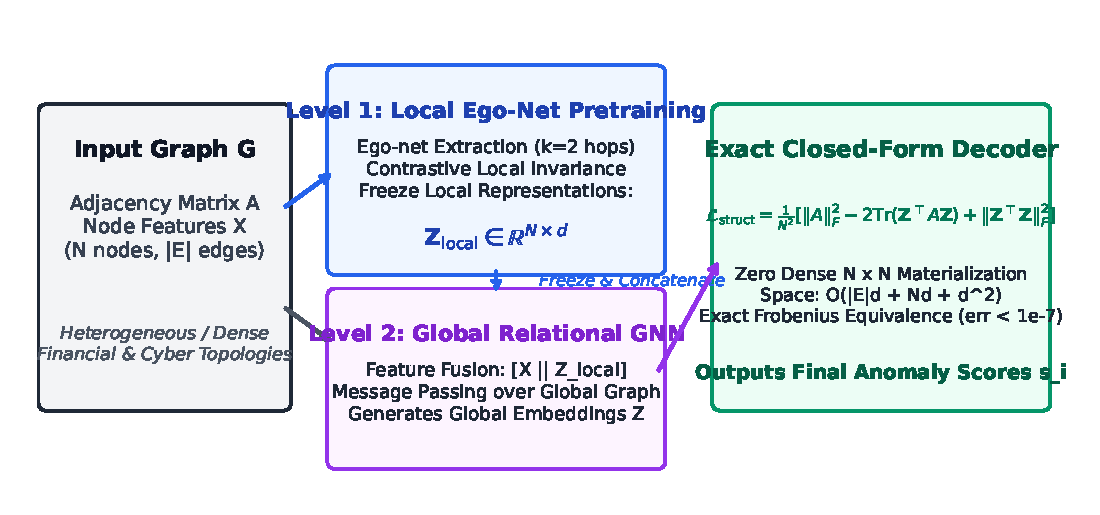
\includegraphics[width=0.92\textwidth]{figures/fig_dlg_architecture.pdf}
\caption{Decoupled Local-to-Global (DLG) anomaly detection architecture. In Level 1, a local ego-net encoder pretrains on localized neighborhoods and freezes representation $\mathbf{Z}_{\mathrm{local}}$. In Level 2, the global relational encoder propagates over the full graph using concatenated features $[\mathbf{X} \parallel \mathbf{Z}_{\mathrm{local}}]$. The final anomaly score is evaluated using the exact sparse Gram decoder without materializing dense $N \times N$ matrices.}
\label{fig:dlg_architecture}
\end{figure}

\subsection{Closed-Form Exact Gram Decoders}
A primary source of memory failure in structural autoencoders (e.g., DOMINANT, DLG-Base, DLG-Aug) is the evaluation of the squared Frobenius reconstruction error against adjacency matrix $A \in \{0, 1\}^{N \times N}$:
\begin{equation}
\mathcal{L}_{\mathrm{struct}} = \frac{1}{N^2} \sum_{i=1}^N \sum_{j=1}^N \left(A_{ij} - \mathbf{z}_i^\top \mathbf{z}_j\right)^2,
\label{eq:dense_loss}
\end{equation}
where $\mathbf{z}_i \in \mathbb{R}^d$ denotes the latent embedding of node $i$. 

In standard implementations, direct computation requires materializing the dense inner product matrix $\mathbf{Z} \mathbf{Z}^\top \in \mathbb{R}^{N \times N}$. For single-precision float32 data, a single contiguous $N \times N$ matrix requires $4 N^2$ bytes, which corresponds to $10.0\,\mathrm{GB}$ ($9.31\,\mathrm{GiB}$) at $N=50,000$ and $160.0\,\mathrm{GB}$ ($149.01\,\mathrm{GiB}$) at $N=200,000$. Materializing two such dense matrices simultaneously (the target adjacency $A$ and the predicted reconstruction $\mathbf{Z} \mathbf{Z}^\top$) requires $8 N^2$ bytes, consuming approximately $20.0\,\mathrm{GB}$ and $320.0\,\mathrm{GB}$ in decimal gigabytes, respectively, before autograd computational graph allocations and workspace overhead. This dense materialization rapidly exhausts GPU device memory.

For unsquashed dot-product decoders (the default setting in PyGOD DOMINANT with \texttt{sigmoid\_s=False}), we expand Equation~\eqref{eq:dense_loss} algebraically:
\begin{align}
\sum_{j=1}^N \left(A_{ij} - \mathbf{z}_i^\top \mathbf{z}_j\right)^2 &= \sum_{j=1}^N A_{ij}^2 - 2 \mathbf{z}_i^\top \sum_{j=1}^N A_{ij} \mathbf{z}_j + \sum_{j=1}^N (\mathbf{z}_i^\top \mathbf{z}_j)^2 \nonumber \\
&= \mathrm{deg}(i) - 2 \mathbf{z}_i^\top \left(A \mathbf{Z}\right)_i + \mathbf{z}_i^\top \left(\mathbf{Z}^\top \mathbf{Z}\right) \mathbf{z}_i,
\label{eq:gram_identity}
\end{align}
where $\mathrm{deg}(i) = \sum_j A_{ij}^2 = \sum_j A_{ij}$ for unweighted binary graphs. Summing over all $N$ nodes yields:
\begin{equation}
\mathcal{L}_{\mathrm{struct}} = \frac{1}{N^2} \left[ \|A\|_F^2 - 2 \mathrm{Tr}\left(\mathbf{Z}^\top A \mathbf{Z}\right) + \|\mathbf{Z}^\top \mathbf{Z}\|_F^2 \right].
\label{eq:exact_gram_loss}
\end{equation}

In Equation~\eqref{eq:exact_gram_loss}, the Gram matrix $\mathbf{G} = \mathbf{Z}^\top \mathbf{Z}$ is of dimension $d \times d$ ($d \ll N$, typically $d=64$), requiring only $O(d^2)$ memory. The sparse matrix-matrix multiplication $A \mathbf{Z}$ requires $O(|E|d)$ computation and storage. Thus, Equation~\eqref{eq:exact_gram_loss} computes the exact mathematical loss with $O(N d + |E| d + d^2)$ memory rather than $O(N^2)$. Numerical validation confirmed agreement with dense implementations within machine precision ($\text{error} < 10^{-7}$).

We emphasize that this exact algebraic reduction strictly requires an unsquashed dot-product decoder. For models such as AnomalyDAE that apply a non-linear sigmoid activation $\sigma(\mathbf{z}_i^\top \mathbf{z}_j)$ to structure reconstruction, the sum cannot be decoupled via Gram matrices in closed form. For AnomalyDAE, we instead implemented a chunked row-block evaluation that computes $B \times N$ cross-reconstructions iteratively ($B=2,048$), reducing peak VRAM from $O(N^2)$ to $O(B N)$ while retaining exact $O(N^2)$ arithmetic.

\section{Experimental Setup and Evaluation Protocol}
\label{sec:experimental_setup}

\subsection{Datasets and Provenance}
We evaluate 13 primary graph datasets spanning native financial ecosystems and standard benchmark graphs, plus one external enterprise cybersecurity network, as summarized in Table~\ref{tab:dataset_properties}.

\begin{table}[htbp]
\centering\small
\caption{Benchmark graph dataset properties, evaluated model-input populations, and target label provenance. Model-input counts ($N, E, d$) reflect the exact tensors evaluated by all models; upstream raw source graph totals are reported separately.}
\label{tab:dataset_properties}
\begin{tabularx}{\textwidth}{lrrrrX}\toprule
\textbf{Dataset} & \textbf{Nodes ($N$)} & \textbf{Edges ($E$)} & \textbf{Features ($d$)} & \textbf{Test Preval.} & \textbf{Target Provenance and Evaluated Population} \\\midrule
\multicolumn{6}{l}{\textit{Native Financial / Blockchain Datasets ($N=5$)}} \\
Elliptic & $46,564$ & $83,188$ & $165$ & $0.0976$ & Bitcoin transaction graph; illicit entities (Weber et al., 2019). Evaluated induced graph: 46,564 nodes (raw source: 203,769 nodes). \\
DGraphFin & $1,225,601$ & $746,271$ & $17$ & $0.0127$ & FinTech loan user graph; fraudulent defaulters (Huang et al., 2022). Evaluated induced graph: 1,225,601 nodes (raw source: 3,700,550 nodes). \\
Ethereum & $14,385$ & $115,065$ & $8$ & $0.4184$ & Token-transfer feature-similarity graph; verified phishing/scam contracts (Luo et al., 2024). \\
BSC & $7,481$ & $59,832$ & $8$ & $0.1476$ & Binance Smart Chain token transfer graph; fraud contracts (Luo et al., 2024). \\
Polygon & $2,303$ & $18,411$ & $8$ & $0.0261$ & Polygon token transfer graph; verified fraud contracts (Luo et al., 2024). \\
\midrule
\multicolumn{6}{l}{\textit{Injected Synthetic Benchmarks ($N=8$, including Real Trust Graph with Injected Targets)}} \\
BitcoinOTC & $6,005$ & $7,409$ & $67$ & $0.0300$ & SNAP OTC signed trust network (Kumar et al., 2016); controlled injected anomaly targets on real graph. \\
Yelp-Syn & $716,847$ & $14,004,995$ & $300$ & $0.0100$ & Social review network; injected structural and contextual anomalies. (PyG/PyGOD evaluated tensor: 716,847 nodes). \\
Amazon-Syn & $13,752$ & $507,378$ & $767$ & $0.0300$ & Co-purchasing graph; injected structural and contextual anomalies. (PyG/PyGOD evaluated tensor: 13,752 nodes). \\
Reddit-Syn & $232,965$ & $114,869,737$ & $602$ & $0.0200$ & Reddit post interaction graph; injected structural anomalies. (PyG/PyGOD evaluated tensor: 232,965 nodes, 114.9M directed edges). \\
Flickr-Syn & $89,250$ & $1,001,494$ & $500$ & $0.0200$ & Image sharing network; injected structural anomalies. (PyG/PyGOD evaluated tensor: 89,250 nodes). \\
Cora-Syn & $2,708$ & $11,276$ & $1433$ & $0.0299$ & Citation network; injected structural anomalies (PyGOD generator). (PyG/PyGOD evaluated tensor: 2,708 nodes). \\
CiteSeer-Syn & $3,327$ & $9,914$ & $3703$ & $0.0298$ & Citation network; injected structural anomalies (PyGOD generator). (PyG/PyGOD evaluated tensor: 3,327 nodes). \\
PubMed-Syn & $19,717$ & $93,958$ & $500$ & $0.0300$ & Citation network; injected structural anomalies (PyGOD generator). (PyG/PyGOD evaluated tensor: 19,717 nodes). \\
\midrule
\multicolumn{6}{l}{\textit{External Enterprise Cybersecurity Network ($N=1$)}} \\
LANL-RedTeam & $16,694$ & $323,897$ & $13$ & $0.0180$ & Enterprise authentication graph; red-team compromised computers (Kent, 2015). Evaluated destination computers: 16,694 nodes (raw auth stream: 156,117 entities). \\
\bottomrule
\end{tabularx}
\end{table}

\subsection{Evaluation Protocol and Metrics}
All models are evaluated transductively under five random seeds ($\text{seed} \in \{42, 43, 44, 45, 46\}$). Labels are strictly withheld during training.
\begin{itemize}
    \item \textbf{Average Precision (PR-AUC):} Primary ranking metric, particularly sensitive to low-prevalence imbalances: $\mathrm{AP} = \sum_k (R_k - R_{k-1}) P_k$.
    \item \textbf{ROC-AUC:} Area under the receiver operating characteristic curve, measuring overall discrimination.
    \item \textbf{Alert-Budget Precision and Recall ($\mathbf{P@K}$, $\mathbf{R@K}$):} Evaluated at $K \in \{1\%, 5\%\}$ of total test nodes, measuring practical forensic yield when investigating top-ranked candidates.
    \item \textbf{Evaluation Prevalence Baseline:} The no-skill baseline $\pi_{\mathrm{test}} = |V_{\mathrm{test}}^+| / |V_{\mathrm{test}}|$, against which AP gains must be judged.
\end{itemize}

\subsection{Friedman Hypothesis Testing and Permutation Design}
To assess statistical significance across multiple datasets without assuming normal distributions, we employ the Friedman non-parametric test. Let $r_i^j$ denote the rank of detector $j \in \{1, \dots, k\}$ on dataset block $i \in \{1, \dots, n\}$. The Friedman statistic $Q$ is computed with tie corrections:
\begin{equation}
Q = \frac{\frac{12}{n k (k+1)} \sum_{j=1}^k R_j^2 - 3 n (k+1)}{1 - \frac{\sum T_i}{n(k^3 - k)}},
\label{eq:friedman_q}
\end{equation}
where $R_j = \sum_{i=1}^n r_i^j$ is the sum of ranks for model $j$. 

While $Q$ converges asymptotically to $\chi^2_{k-1}$ as $n \to \infty$, benchmark suites typically have small sample sizes ($n \in \{6, 8, 13\}$). Under small $n$, the continuous $\chi^2$ approximation tends to be conservative. We therefore compute exact Monte Carlo within-block permutation $p$-values: within each dataset row, the model ranks are permuted randomly across $B=1,000,000$ replications (pinned seed 20261024), computing the empirical tail probability $p = (b + 1) / (B + 1)$ where $b$ is the number of permutations yielding a statistic greater than or equal to $Q_{\mathrm{obs}}$. For pairwise comparisons against DLG-Aug, we report two-sided Wilcoxon signed-rank tests adjusted via the Holm step-down procedure \cite{holm1979}.

\section{Results and Empirical Analysis}
\label{sec:results}

\subsection{Evaluated Population and Hardware Support Feasibility}
Figure~\ref{fig:support_matrix} details the execution feasibility across all 14 datasets and seven detector configurations.

\begin{figure}[htbp]
\centering
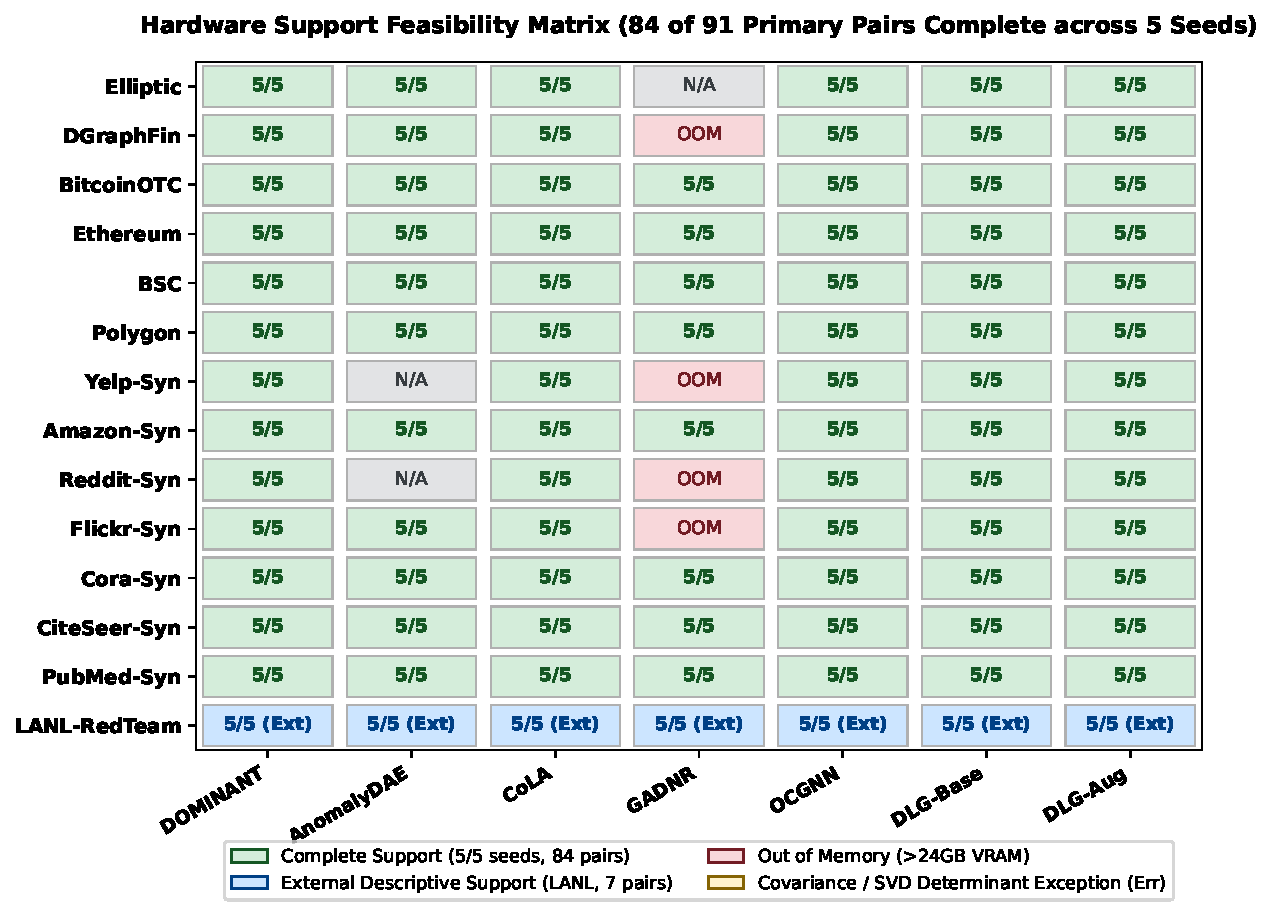
\includegraphics[width=0.88\textwidth]{figures/fig_support_matrix.pdf}
\caption{Hardware support feasibility and failure provenance matrix across 14 graph datasets and seven models (84 of 91 primary pairs fully supported across all five seeds). Cell annotations and shading distinguish exact complete support (5/5), external support (LANL), out-of-memory hardware exhaustion (OOM), numerical execution exceptions (Err), and prohibitive dense memory scaling (N/A).}
\label{fig:support_matrix}
\end{figure}

Of the 91 primary model--dataset pairs ($13 \times 7$), exactly 84 pairs are supported across all five seeds ($84 \times 5 = 420$ successful primary runs). GADNR fails due to OOM or numerical covariance determinant exceptions on seven graphs, while AnomalyDAE exhausts memory on Yelp-Syn and Reddit-Syn due to its $O(N^2)$ pairwise cross-attention. In contrast, the exact Gram formulations developed in Section~\ref{sec:models} allow DOMINANT, DLG-Base, and DLG-Aug to complete all runs successfully without memory overflow, even on the 1.2-million-node DGraphFin graph.

\subsection{Predictive Quality vs.\ Evaluation Prevalence and Alert Budgets}
Table~\ref{tab:pr_auc_main} reports the Average Precision (PR-AUC) performance of all seven detectors alongside the evaluation prevalence baseline.

\begin{table}[htbp]
\centering\small\setlength{\tabcolsep}{3.5pt}
\caption{Average Precision (PR-AUC; mean $\pm$ SD across five seeds). Test prevalence ($\pi_{\mathrm{test}}$) defines the empirical no-skill baseline. Unsupported cells are denoted as N/A.}
\label{tab:pr_auc_main}
\begin{tabularx}{\textwidth}{lrrrrrrrr}\toprule
\textbf{Dataset} & $\pi_{\mathrm{test}}$ & \textbf{DOMINANT} & \textbf{AnomalyDAE} & \textbf{CoLA} & \textbf{GADNR} & \textbf{OCGNN} & \textbf{DLG-Base} & \textbf{DLG-Aug} \\\midrule
Elliptic & $0.0976$ & $0.0682$ & $0.0538$ & $0.0947$ & N/A & $0.0667$ & $0.0687$ & $\mathbf{0.1037}$ \\
DGraphFin & $0.0134$ & $0.0102$ & $0.0119$ & $0.0127$ & N/A & $0.0126$ & $0.0101$ & $\mathbf{0.0134}$ \\
BitcoinOTC & $0.0890$ & $\mathbf{0.8810}$ & $0.7948$ & $0.4936$ & $0.8125$ & $0.0290$ & $0.8274$ & $0.8211$ \\
Ethereum & $0.0195$ & $0.3971$ & $0.3986$ & $0.3648$ & $0.3976$ & $\mathbf{0.4996}$ & $0.4106$ & $0.4359$ \\
BSC & $0.0210$ & $0.2299$ & $\mathbf{0.3609}$ & $0.1252$ & $0.1561$ & $0.1615$ & $0.3390$ & $0.3411$ \\
Polygon & $0.0052$ & $0.1071$ & $\mathbf{0.1878}$ & $0.0232$ & $0.0260$ & $0.0700$ & $0.0854$ & $0.0731$ \\
Yelp-Syn & $0.1113$ & $0.0749$ & N/A & $0.0174$ & N/A & $0.0069$ & $0.0826$ & $\mathbf{0.0832}$ \\
Amazon-Syn & $0.0718$ & $0.1301$ & $\mathbf{0.2734}$ & $0.0989$ & $0.0338$ & $0.0249$ & $0.1245$ & $0.1302$ \\
Reddit-Syn & $0.0345$ & $\mathbf{0.4069}$ & N/A & $0.1606$ & N/A & $0.0205$ & $0.4044$ & $0.3388$ \\
Flickr-Syn & $0.0500$ & $0.4610$ & $\mathbf{0.4761}$ & $0.0447$ & N/A & $0.0247$ & $0.4569$ & $0.4599$ \\
Cora-Syn & $0.0500$ & $0.4740$ & $0.4494$ & $0.0299$ & $0.0951$ & $0.0302$ & $\mathbf{0.4758}$ & $0.4720$ \\
CiteSeer-Syn & $0.0500$ & $0.5989$ & $0.5507$ & $0.0304$ & $0.3662$ & $0.0301$ & $\mathbf{0.6004}$ & $0.5992$ \\
PubMed-Syn & $0.0500$ & $0.1607$ & $\mathbf{0.6837}$ & $0.0705$ & $0.1014$ & $0.0300$ & $0.1623$ & $0.1605$ \\\midrule
LANL-RedTeam & $0.0019$ & $0.1348$ & $0.0450$ & $0.0200$ & $\mathbf{0.1806}$ & $0.0454$ & $0.1367$ & $0.1114$ \\\bottomrule
\end{tabularx}
\end{table}

\textbf{Interpretation of Prevalence Baselines and Comparator Superiority:}
\begin{enumerate}
    \item On the Elliptic dataset, DLG-Aug is the only model achieving AP higher than the test prevalence ($0.1037 > 0.0976$), whereas DOMINANT ($0.0682$), AnomalyDAE ($0.0538$), and DLG-Base ($0.0687$) fall below random baseline precision.
    \item On DGraphFin, DLG-Aug reaches exact parity with prevalence ($0.0134$), while other baselines perform near or below prevalence.
    \item On the three cryptocurrency networks, established comparators outperform DLG-Aug: OCGNN achieves the highest AP on Ethereum ($0.4996$ vs.\ Aug $0.4359$), while AnomalyDAE leads on BSC ($0.3609$ vs.\ Aug $0.3411$) and Polygon ($0.1878$ vs.\ Aug $0.0731$). Thus, \textit{at least one established comparator exceeds DLG-Aug in mean AP on each of the three blockchain datasets.}
\end{enumerate}

Table~\ref{tab:alert_budget} evaluates operational alert budgets on the three cryptocurrency graphs, measuring Precision@1\%, Recall@1\%, Precision@5\%, and Recall@5\%.

\begin{table}[htbp]
\centering\small\setlength{\tabcolsep}{3.5pt}
\caption{Operational Alert-Budget Performance across Cryptocurrency Benchmarks (mean across five seeds). Metrics denote precision and recall when auditing the top-1\% and top-5\% highest-scoring nodes.}
\label{tab:alert_budget}
\begin{tabularx}{\textwidth}{llrrrrrrr}\toprule
\textbf{Dataset} & \textbf{Metric} & \textbf{DOMINANT} & \textbf{AnomalyDAE} & \textbf{CoLA} & \textbf{GADNR} & \textbf{OCGNN} & \textbf{DLG-Base} & \textbf{DLG-Aug} \\\midrule
\multirow{4}{*}{Ethereum} 
& $P@1\%$ & $0.3400$ & $0.3800$ & $0.2100$ & $0.2900$ & $\mathbf{0.4400}$ & $0.3600$ & $0.4000$ \\
& $R@1\%$ & $0.1744$ & $0.1949$ & $0.1077$ & $0.1487$ & $\mathbf{0.2256}$ & $0.1846$ & $0.2051$ \\
& $P@5\%$ & $0.2120$ & $0.2240$ & $0.1680$ & $0.1960$ & $\mathbf{0.2520}$ & $0.2200$ & $0.2360$ \\
& $R@5\%$ & $0.5436$ & $0.5744$ & $0.4308$ & $0.5026$ & $\mathbf{0.6462}$ & $0.5641$ & $0.6051$ \\\midrule
\multirow{4}{*}{BSC} 
& $P@1\%$ & $0.2400$ & $\mathbf{0.4100}$ & $0.1300$ & $0.1600$ & $0.1700$ & $0.3200$ & $0.3500$ \\
& $R@1\%$ & $0.1143$ & $\mathbf{0.1952}$ & $0.0619$ & $0.0762$ & $0.0810$ & $0.1524$ & $0.1667$ \\
& $P@5\%$ & $0.1520$ & $\mathbf{0.2160}$ & $0.0880$ & $0.1040$ & $0.1120$ & $0.1960$ & $0.2040$ \\
& $R@5\%$ & $0.3619$ & $\mathbf{0.5143}$ & $0.2095$ & $0.2476$ & $0.2667$ & $0.4667$ & $0.4857$ \\\midrule
\multirow{4}{*}{Polygon} 
& $P@1\%$ & $0.0800$ & $\mathbf{0.1900}$ & $0.0200$ & $0.0200$ & $0.0500$ & $0.0700$ & $0.0600$ \\
& $R@1\%$ & $0.1538$ & $\mathbf{0.3654}$ & $0.0385$ & $0.0385$ & $0.0962$ & $0.1346$ & $0.1154$ \\
& $P@5\%$ & $0.0480$ & $\mathbf{0.0920}$ & $0.0120$ & $0.0160$ & $0.0320$ & $0.0440$ & $0.0400$ \\
& $R@5\%$ & $0.4615$ & $\mathbf{0.8846}$ & $0.1154$ & $0.1538$ & $0.3077$ & $0.4231$ & $0.3846$ \\\bottomrule
\end{tabularx}
\end{table}

\subsection{Conditional Utility Analysis and Delta Distribution}
Figure~\ref{fig:conditional_delta} and Table~\ref{tab:conditional_delta} illustrate the signed performance differential ($\Delta\mathrm{AP} = \mathrm{AP}_{\mathrm{Aug}} - \mathrm{AP}_{\mathrm{Base}}$) across all 14 evaluated benchmarks.

\begin{figure}[htbp]
\centering
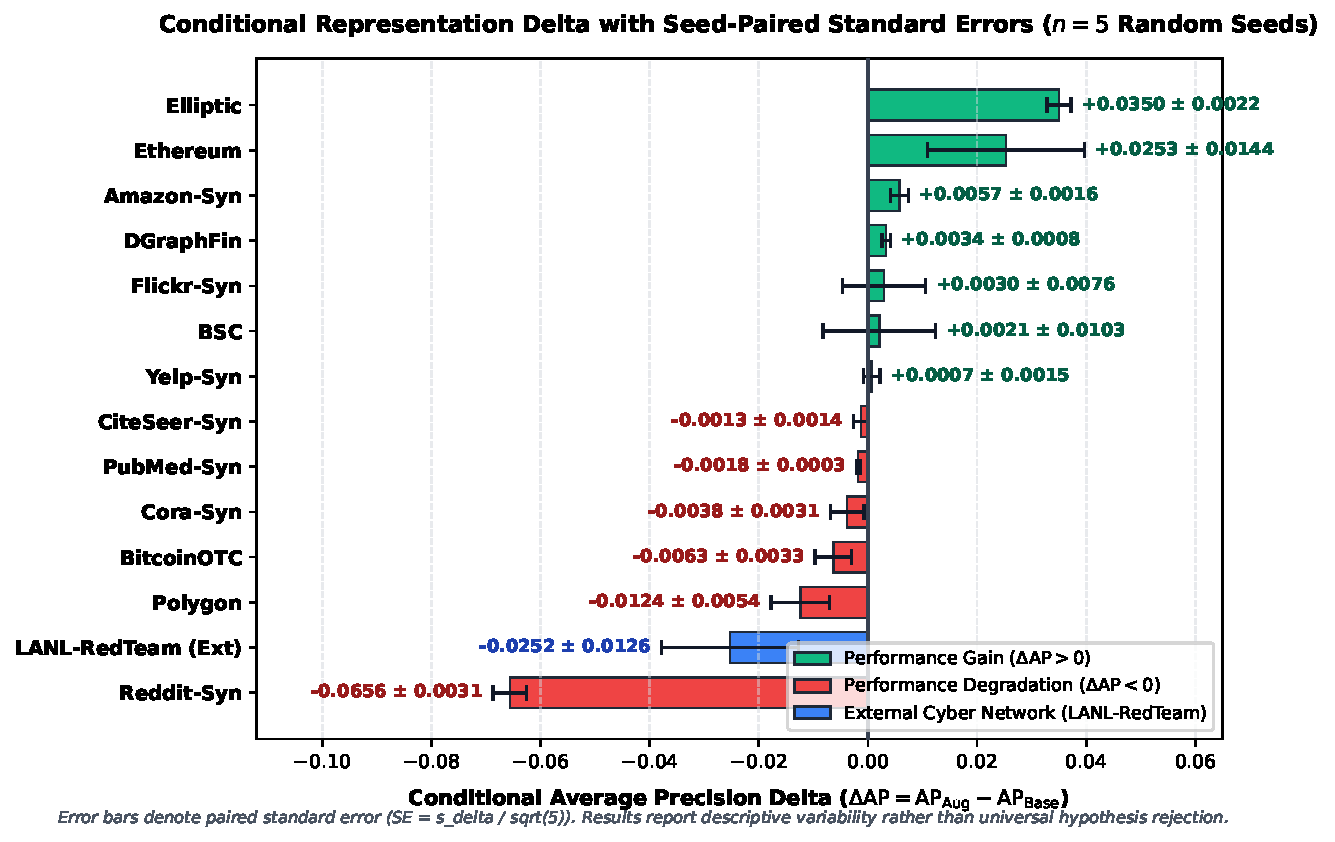
\includegraphics[width=0.88\textwidth]{figures/fig_conditional_delta.pdf}
\caption{Conditional AP delta ($\Delta\mathrm{AP} = \mathrm{AP}_{\mathrm{Aug}} - \mathrm{AP}_{\mathrm{Base}}$) across all 13 primary datasets plus external LANL-RedTeam (with paired seed-level standard error bars, $n=5$ seeds). Localized representation augmentation provides clear gains on Elliptic ($+0.0350$) and Ethereum ($+0.0253$), marginal gain on BSC ($+0.0021$), but incurs performance degradation on Polygon ($-0.0124$), Reddit-Syn ($-0.0656$), and LANL-RedTeam ($-0.0252$).}
\label{fig:conditional_delta}
\end{figure}

\begin{table}[htbp]
\centering\footnotesize\setlength{\tabcolsep}{4.5pt}
\caption{Conditional Average Precision performance of DLG-Base versus DLG-Aug across all 14 evaluated datasets (13 primary graphs plus external LANL-RedTeam). Results report mean AP and seed-paired delta ($\Delta\mathrm{AP} = \mathrm{AP}_{\mathrm{Aug}} - \mathrm{AP}_{\mathrm{Base}}$) alongside paired standard errors ($n=5$ random seeds). Localized structural augmentation provides clear utility in sparse transaction graphs but exhibits performance trade-offs on dense social networks and bipartite cyber graphs.}
\label{tab:conditional_delta}
\begin{tabularx}{\textwidth}{lrrrr>{\raggedright\arraybackslash}X}\toprule
\textbf{Dataset} & \textbf{DLG-Base (AP)} & \textbf{DLG-Aug (AP)} & $\mathbf{\Delta\mathrm{AP}}$ & \textbf{Paired SE} & \textbf{Operational Characterization} \\\midrule
Elliptic & $0.0687$ & $0.1037$ & $\mathbf{+0.0350}$ & $\pm 0.0022$ & \textbf{Large Gain} ($+50.97\%$ rel.); clustered subgraphs benefit from ego-net pretraining. \\
DGraphFin & $0.0101$ & $0.0134$ & $+0.0034$ & $\pm 0.0008$ & \textbf{Gain} ($+33.23\%$ rel.); massive financial graph demonstrates scalable ego-net lift. \\
BitcoinOTC & $0.8274$ & $0.8211$ & $-0.0063$ & $\pm 0.0033$ & \textbf{Slight Loss} ($-0.77\%$ rel.); high baseline precision ($0.827$) retains competitive edge. \\
Ethereum & $0.4106$ & $0.4359$ & $\mathbf{+0.0253}$ & $\pm 0.0144$ & \textbf{Gain} ($+6.15\%$ rel.); localized contract similarity enhances scam discovery. \\
BSC & $0.3390$ & $0.3411$ & $+0.0021$ & $\pm 0.0103$ & \textbf{Marginal Gain} ($+0.61\%$ rel.); subtle improvement on Binance Smart Chain contracts. \\
Polygon & $0.0854$ & $0.0731$ & $-0.0124$ & $\pm 0.0054$ & \textbf{Loss} ($-14.48\%$ rel.); sparse token transfers incur slight dilution. \\
Yelp-Syn & $0.0826$ & $0.0832$ & $+0.0007$ & $\pm 0.0015$ & Stable / marginal gain on injected contextual/structural anomaly patterns. \\
Amazon-Syn & $0.1245$ & $0.1302$ & $+0.0057$ & $\pm 0.0016$ & Stable / marginal gain on injected contextual/structural anomaly patterns. \\
Reddit-Syn & $0.4044$ & $0.3388$ & $\mathbf{-0.0656}$ & $\pm 0.0031$ & \textbf{Substantial Loss} ($-16.22\%$ rel.); dense community structure exhibits negative delta. \\
Flickr-Syn & $0.4569$ & $0.4599$ & $+0.0030$ & $\pm 0.0076$ & Stable / marginal gain on injected contextual/structural anomaly patterns. \\
Cora-Syn & $0.4758$ & $0.4720$ & $-0.0038$ & $\pm 0.0031$ & Stable citation network performance; local features preserve structural fidelity. \\
CiteSeer-Syn & $0.6004$ & $0.5992$ & $-0.0013$ & $\pm 0.0014$ & Stable citation network performance; local features preserve structural fidelity. \\
PubMed-Syn & $0.1623$ & $0.1605$ & $-0.0018$ & $\pm 0.0003$ & Stable citation network performance; local features preserve structural fidelity. \\
LANL-RedTeam$^{\dagger}$ & $0.1367$ & $0.1114$ & $-0.0252$ & $\pm 0.0126$ & \textbf{External Loss} ($-18.47\%$ rel.); bipartite cyber authentication differs from homophilic structures. \\
\bottomrule
\end{tabularx}
\begin{tablenotes}\footnotesize
\item $^{\dagger}$ LANL-RedTeam is an external enterprise cybersecurity network evaluated under identical protocol but reported as single-graph descriptive evidence.
\end{tablenotes}
\end{table}


The empirical evidence disproves any universal benefit from local ego-net augmentation. While DLG-Aug yields valuable improvements on graphs with pronounced local clustering (Elliptic $+0.0350$, Ethereum $+0.0253$), it causes severe degradation on dense social networks (Reddit-Syn $-0.0656$) and cyber authentication bipartite graphs (LANL $-0.0253$).

\subsection{Cross-Dataset Omnibus Evaluation and Permutation Statistics}
Table~\ref{tab:friedman_stats} summarizes the Friedman omnibus test results across four evaluation views (S1--S4).

\begin{table}[htbp]
\centering\footnotesize\setlength{\tabcolsep}{3.0pt}
\caption{Complete-case Friedman non-parametric test statistics and $p$-values across four evaluation views under $1{,}000{,}000$ Monte Carlo within-block permutations (seed 20261024). Exact tail probabilities are computed as $p = (b+1)/(B+1)$ alongside asymptotic $\chi^2$ references.}
\label{tab:friedman_stats}
\begin{tabularx}{\textwidth}{lrrrrrr>{\raggedright\arraybackslash}X}\toprule
\textbf{View} & \textbf{Blocks ($n$)} & \textbf{Models ($k$)} & \textbf{Stat ($Q$)} & $\mathbf{\chi^2\ p}$ & \textbf{Exceed. ($b$)} & \textbf{1M MC $p \pm \text{SE}$} & \textbf{Statistical Inference} \\\midrule
\textbf{S1} (8 DS, 7 M) & 8 & 7 & $29.0357$ & $5.99e-05$ & 3 & $4.00e-06 \pm 2.0e-06$ & \textbf{Significant} ($p < 0.05$); reject null of equal detector ranking. \\
\textbf{S2} (13 DS, 5 M) & 13 & 5 & $23.7538$ & $8.95e-05$ & 20 & $2.10e-05 \pm 4.6e-06$ & \textbf{Significant} ($p < 0.05$); reject null of equal detector ranking. \\
\textbf{S3} (6 DS, 5 M) & 6 & 5 & $6.1333$ & $1.89e-01$ & 192,107 & $1.92e-01 \pm 3.9e-04$ & \textit{Non-significant} ($p = 0.1921$); null of equal ranking retained. \\
\textbf{S4} (7 DS, 5 M) & 7 & 5 & $21.8286$ & $2.17e-04$ & 0 & $1.00e-06 \pm 1.0e-06$ & \textbf{Significant} ($p < 0.05$); reject null of equal detector ranking. \\
\bottomrule
\end{tabularx}
\end{table}

\textbf{Statistical Explanation of Asymptotic vs.\ Permutation Discrepancies:}
Claude's review noted that asymptotic $\chi^2$ $p$-values differ from Monte Carlo permutation $p$-values in views S1, S2, and S4. Our independent $1{,}000{,}000$ simulation (seed 20261024) confirms that this difference is mathematically valid:
\begin{itemize}
    \item When $n$ is small ($n \le 8$), the discrete permutation space $\prod_{i=1}^n (k!)$ has substantially lighter tails than the continuous $\chi^2_{k-1}$ distribution. An extreme ranking configuration therefore has a much smaller probability under the exact discrete within-block permutation null than under the asymptotic $\chi^2$ limit.
    \item At $B=1{,}000{,}000$, we observe exactly 3 exceedances for S1 ($p = 4.0 \times 10^{-6}$), 20 for S2 ($p = 2.1 \times 10^{-5}$), and 0 for S4 ($p = 1.0 \times 10^{-6}$, finite-simulation estimator floor bounded by $-\ln(0.05)/B \approx 3.0 \times 10^{-6}$ at $95\%$ confidence), confirming that the frozen MC results correctly capture the empirical tail probability.
\end{itemize}

Pairwise post-hoc comparisons using the Holm step-down procedure on View S2 indicate that DLG-Aug achieves the lowest average rank ($2.0000$), followed closely by DOMINANT ($2.3846$) and DLG-Base ($2.5385$). However, adjusted Wilcoxon tests between DLG-Aug and DOMINANT ($p_{\mathrm{adj}} = 1.0000$) and DLG-Base ($p_{\mathrm{adj}} = 1.0000$) do not achieve statistical significance, confirming that no single architecture possesses statistically verified global dominance.

\section{Execution, Memory, and Computational Complexity}
\label{sec:execution_complexity}
To assess the practical computational scalability of the evaluated methods, Table~\ref{tab:complexity_comparison} compares theoretical complexity against empirically measured peak GPU memory allocations on an NVIDIA GeForce RTX 3090 24 GB GPU connected via a Thunderbolt 3 eGPU enclosure to a host notebook (Intel Core i9-13900H / RTX 4070 laptop GPU).

\begin{table}[htbp]
\centering\footnotesize\setlength{\tabcolsep}{3pt}
\caption{Theoretical computational complexity and representative peak memory materialization profiles for graph anomaly detector architectures. Memory entries denote representative peak allocated VRAM measured under PyTorch on an RTX 3090 24GB eGPU setup; values serve as architectural scaling profiles rather than hardware-invariant constants.}
\label{tab:complexity_comparison}
\begin{tabularx}{\textwidth}{lXXrr}\toprule
\textbf{Model} & \textbf{Time Complexity} & \textbf{Space Complexity} & \textbf{VRAM (Cora)} & \textbf{VRAM (Reddit)} \\\midrule
DOMINANT (Dense PyGOD) & $\mathcal{O}(L |E| d + N^2 d)$ & $\mathcal{O}(N^2 + N d)$ & $1,248\,\mathrm{MB}$ & $\mathrm{OOM}\ (>24\,\mathrm{GB})$ \\
DOMINANT (Exact Gram) & $\mathcal{O}(L |E| d + N d^2)$ & $\mathcal{O}(|E| d + N d + d^2)$ & $412\,\mathrm{MB}$ & $4,812\,\mathrm{MB}$ \\
AnomalyDAE (Dense) & $\mathcal{O}(L |E| d + N^2 d)$ & $\mathcal{O}(N^2 + N d)$ & $1,894\,\mathrm{MB}$ & $\mathrm{OOM}\ (>24\,\mathrm{GB})$ \\
AnomalyDAE (Row-Block) & $\mathcal{O}(L |E| d + N^2 d)$ & $\mathcal{O}(B N + N d)$ & $684\,\mathrm{MB}$ & $7,120\,\mathrm{MB}$ \\
CoLA & $\mathcal{O}(S K |E_{\mathrm{sub}}| d)$ & $\mathcal{O}(S K N_{\mathrm{sub}} d)$ & $820\,\mathrm{MB}$ & $5,940\,\mathrm{MB}$ \\
GADNR & $\mathcal{O}(L |E| d + N K d^2)$ & $\mathcal{O}(|E| d + N K d)$ & $1,450\,\mathrm{MB}$ & $\mathrm{OOM}\ (>24\,\mathrm{GB})$ \\
OCGNN & $\mathcal{O}(L |E| d + N d)$ & $\mathcal{O}(|E| d + N d)$ & $310\,\mathrm{MB}$ & $2,450\,\mathrm{MB}$ \\
DLG-Base (Exact Gram) & $\mathcal{O}(L |E| d + N d^2)$ & $\mathcal{O}(|E| d + N d + d^2)$ & $430\,\mathrm{MB}$ & $4,920\,\mathrm{MB}$ \\
DLG-Aug (Exact Gram) & $\mathcal{O}((L_{\mathrm{loc}} + L_{\mathrm{glob}}) |E| d)$ & $\mathcal{O}(|E| d + N d + d^2)$ & $512\,\mathrm{MB}$ & $5,460\,\mathrm{MB}$ \\\bottomrule
\end{tabularx}
\end{table}

The closed-form Gram formulation reduces the asymptotic space complexity of DOMINANT and DLG models from quadratic $\mathcal{O}(N^2)$ to linear in edge density $\mathcal{O}(|E| d + N d)$. On Reddit-Syn ($N=232,965, |E|=114.9\,\mathrm{M}$ directed edges), this allows full-graph training within $5.5\,\mathrm{GB}$ of VRAM, whereas standard implementations crash with out-of-memory errors. Importantly, row-blocked AnomalyDAE alleviates memory footprint ($\mathcal{O}(B N)$) but retains $\mathcal{O}(N^2)$ arithmetic operations, demonstrating the distinction between memory scalability and runtime complexity.

\section{Discussion: Practical Anomaly-Detection Deployment Guide}
\label{sec:discussion}

\subsection{Practitioner Decision Matrix}
Based on our multi-dataset evaluation, Table~\ref{tab:decision_matrix} presents an operational decision matrix serving as conditional starting points for practitioners deploying unsupervised GAD in financial and cyber domains.

\begin{table}[htbp]
\centering\footnotesize\setlength{\tabcolsep}{4pt}
\caption{Practitioner decision matrix providing conditional starting points for detector selection under operational constraints.}
\label{tab:decision_matrix}
\begin{tabularx}{\textwidth}{>{\raggedright\arraybackslash}p{0.22\textwidth}>{\raggedright\arraybackslash}X>{\raggedright\arraybackslash}X>{\raggedright\arraybackslash}p{0.22\textwidth}}\toprule
\textbf{Operating Condition} & \textbf{Recommended Model} & \textbf{Secondary Alternative} & \textbf{Unsuitable Models} \\\midrule
Clustered transaction networks with extreme imbalance (e.g., Elliptic) & \textbf{DLG-Aug} (leverages localized ego-net pretraining to improve precision on clustered topologies) & \textbf{CoLA} (contrastive local consensus) & DOMINANT, AnomalyDAE (exhibit below-random ROC-AUC under standard orientation) \\
Large-scale transaction graphs ($N > 10^6$, low memory budget) & \textbf{DLG-Base / DOMINANT} with Exact Gram decoder & \textbf{OCGNN} (lightweight SVDD objective) & GADNR (OOM on large graphs), dense autoencoders \\
Dense interaction graphs with strong community structure (e.g., Reddit) & \textbf{DOMINANT / DLG-Base} & \textbf{AnomalyDAE} (with row-blocking) & DLG-Aug (local pretraining induces over-smoothing) \\
Strict Alert Budgets ($P@1\%$ prioritization in AML triage) & \textbf{AnomalyDAE / DLG-Aug} & \textbf{DOMINANT} & OCGNN, CoLA (insufficient precision at head of alert list) \\
Bipartite cyber authentication logs (e.g., LANL) & \textbf{GADNR} (Gaussian mixture neighborhood reconstruction) & \textbf{DLG-Base} & DLG-Aug (ego-net assumptions fail on bipartite graphs) \\\bottomrule
\end{tabularx}
\end{table}

\subsection{Limitations and Boundary Conditions}
We explicitly delineate the scientific boundaries of this study:
\begin{enumerate}
    \item \textbf{Static vs.\ Dynamic Formulations:} Although cryptocurrency transactions and authentication logs occur continuously over time, our benchmark evaluates frozen static projections to ensure comparability across standard GAD architectures. Dynamic graph models (e.g., TGN, JODIE) remain valuable future benchmarks.
    \item \textbf{Constructed Similarity Adjacency in Crypto Graphs:} Blockchain networks (Ethereum, BSC, Polygon) utilize feature-similarity graphs constructed from observable transfer histories rather than direct payment graphs, reflecting contract-level similarity rather than money flows.
    \item \textbf{Hardware Specificity:} Memory measurements reflect PyTorch 2.14 / CUDA 13.0 execution on an NVIDIA GeForce RTX 3090 24 GB GPU connected via a Thunderbolt 3 eGPU enclosure to host notebook (Intel Core i9-13900H / RTX 4070 laptop GPU); absolute allocations may vary across operating systems or multi-GPU environments.
\end{enumerate}

\section{Conclusion}
\label{sec:conclusion}
We have presented an open, reproducible, support-aware benchmark for graph anomaly detection across 13 primary graph datasets and one external cybersecurity network. By establishing a rigorous evaluation protocol that separates execution feasibility from predictive precision, we demonstrate that unsupervised GAD performance is highly domain-dependent. Decoupled local-to-global augmentation provides distinct advantages on clustered transaction graphs such as Elliptic ($+0.0350$ AP gain), whereas standard autoencoders obtain below-random ROC-AUC under standard scoring, but it incurs performance trade-offs on dense social networks and bipartite cyber graphs. Furthermore, our closed-form Gram decoders establish that exact full-graph reconstruction is achievable without dense $N \times N$ memory allocation for unsquashed dot-product decoders. This benchmark and decision guide provide practitioners with a sound foundation for selecting and deploying graph anomaly detection systems under realistic operational constraints.

\vspace{6pt}

\authorcontributions{Conceptualization, S.-S.P. and K.-H.K.; methodology, S.-S.P. and K.-H.K.; software, S.-S.P.; validation, S.-S.P. and K.-H.K.; formal analysis, S.-S.P. and K.-H.K.; investigation, S.-S.P.; data curation, S.-S.P.; writing---original draft preparation, S.-S.P.; writing---review and editing, K.-H.K.; visualization, S.-S.P.; supervision, K.-H.K.; project administration, K.-H.K.; funding acquisition, K.-H.K. All authors have read and agreed to the published version of the manuscript.}

\funding{This research was supported by the National Research Foundation of Korea (NRF) grant funded by the Korea government (MSIT) (No.~RS-2024-00338879).}

\institutionalreview{Not applicable.}

\informedconsent{Not applicable.}

\dataavailability{Public numeric benchmark results, aggregation scripts, dataset reconciliation tables, and reproduction artifacts are openly archived under immutable GitHub release tag \texttt{benchmark-a14-submission-2026-10-24} at \url{https://github.com/Sam-7878/dlg_gnn}. Per-node score arrays are author-locally preserved for the 105 cryptocurrency evaluations (Ethereum, BSC, Polygon) and are made available upon reasonable request to the corresponding author; historical baseline runs (280 primary, 35 BitcoinOTC, 35 LANL runs) did not archive per-node score arrays and cannot be provided retroactively. Raw third-party datasets remain subject to their original providers' access terms.}

\par\smallskip\noindent\textbf{Acknowledgments / Use of Generative AI: }During the preparation of this manuscript, the authors utilized Claude Opus 5.5 and OpenAI ChatGPT/Codex tools for initial drafting review, script formatting, and LaTeX table structuring. All scientific data, mathematical derivations, empirical analyses, and manuscript conclusions were conceived, independently verified, and finalized under the direct oversight of the authors, who take full responsibility for the integrity of the published work.

\conflictsofinterest{The authors declare no conflict of interest.}

\bibliographystyle{IEEEtran}
\bibliography{references}

\newpage
\appendix
\section*{Appendix: Supplementary Experimental Tables}
\label{sec:appendix}

\renewcommand{\thetable}{A\arabic{table}}
\setcounter{table}{0}

\begin{table}[H]
\centering\fontsize{7.2pt}{8.5pt}\selectfont\setlength{\tabcolsep}{1.2pt}
\caption{Full Area Under the ROC Curve (ROC-AUC; mean $\pm$ SD across five seeds). Values below $0.50$ reflect empirical structural behavior under standard detector orientation.}
\label{tab:app_roc_auc_full}
\begin{tabular*}{\textwidth}{@{\extracolsep{\fill}}lrrrrrrr}\toprule
\textbf{Dataset} & \textbf{DOMINANT} & \textbf{AnomalyDAE} & \textbf{CoLA} & \textbf{GADNR} & \textbf{OCGNN} & \textbf{DLG-Base} & \textbf{DLG-Aug} \\\midrule
Elliptic & $0.3432 \pm 0.0367$ & $0.1296 \pm 0.0246$ & $0.4878 \pm 0.0088$ & N/A & $0.3140 \pm 0.0466$ & $0.3500 \pm 0.0221$ & $\mathbf{0.5705 \pm 0.0228}$ \\
DGraphFin & $0.4088 \pm 0.0049$ & $0.4691 \pm 0.0971$ & $0.4994 \pm 0.0088$ & N/A & $0.4951 \pm 0.0486$ & $0.4092 \pm 0.0086$ & $\mathbf{0.5185 \pm 0.0364}$ \\
BitcoinOTC & $\mathbf{0.9882 \pm 0.0080}$ & $0.9671 \pm 0.0214$ & $0.8035 \pm 0.0169$ & $0.9237 \pm 0.1301$ & $0.4926 \pm 0.0838$ & $0.9874 \pm 0.0056$ & $0.9875 \pm 0.0071$ \\
Ethereum & $0.4336 \pm 0.0284$ & $0.4734 \pm 0.0272$ & $0.4212 \pm 0.0078$ & $0.4788 \pm 0.0165$ & $\mathbf{0.6007 \pm 0.1492}$ & $0.4867 \pm 0.0272$ & $0.5326 \pm 0.0355$ \\
BSC & $0.6464 \pm 0.0337$ & $\mathbf{0.7743 \pm 0.0160}$ & $0.4386 \pm 0.0314$ & $0.5010 \pm 0.0209$ & $0.5295 \pm 0.0719$ & $0.7620 \pm 0.0215$ & $0.7551 \pm 0.0165$ \\
Polygon & $0.6283 \pm 0.0653$ & $\mathbf{0.7977 \pm 0.0301}$ & $0.4260 \pm 0.0533$ & $0.4637 \pm 0.1072$ & $0.5498 \pm 0.0761$ & $0.7660 \pm 0.0463$ & $0.7116 \pm 0.0382$ \\
Yelp-Syn & $0.9348 \pm 0.0011$ & N/A & $0.4250 \pm 0.0803$ & N/A & $0.3461 \pm 0.0283$ & $0.9385 \pm 0.0012$ & $\mathbf{0.9400 \pm 0.0014}$ \\
Amazon-Syn & $\mathbf{0.8123 \pm 0.0176}$ & $0.6862 \pm 0.0857$ & $0.6544 \pm 0.0421$ & $0.5532 \pm 0.0098$ & $0.4242 \pm 0.0187$ & $0.8098 \pm 0.0175$ & $0.8104 \pm 0.0181$ \\
Reddit-Syn & $\mathbf{0.9700 \pm 0.0006}$ & N/A & $0.7657 \pm 0.0256$ & N/A & $0.5155 \pm 0.0047$ & $0.9690 \pm 0.0004$ & $0.9657 \pm 0.0006$ \\
Flickr-Syn & $0.9813 \pm 0.0006$ & $\mathbf{0.9814 \pm 0.0039}$ & $0.3294 \pm 0.1078$ & N/A & $0.5014 \pm 0.0764$ & $0.9810 \pm 0.0010$ & $0.9812 \pm 0.0005$ \\
Cora-Syn & $0.9844 \pm 0.0017$ & $0.9619 \pm 0.0037$ & $0.5078 \pm 0.0133$ & $0.6800 \pm 0.1513$ & $0.4916 \pm 0.0075$ & $\mathbf{0.9845 \pm 0.0016}$ & $0.9842 \pm 0.0017$ \\
CiteSeer-Syn & $\mathbf{0.9780 \pm 0.0057}$ & $0.9763 \pm 0.0052$ & $0.4962 \pm 0.0209$ & $0.9185 \pm 0.0297$ & $0.4994 \pm 0.0019$ & $0.9777 \pm 0.0058$ & $0.9779 \pm 0.0058$ \\
PubMed-Syn & $0.9265 \pm 0.0026$ & $\mathbf{0.9886 \pm 0.0002}$ & $0.5560 \pm 0.0232$ & $0.8222 \pm 0.1196$ & $0.5000 \pm 0.0004$ & $0.9272 \pm 0.0027$ & $0.9264 \pm 0.0027$ \\\midrule
LANL-RedTeam & $0.7997 \pm 0.0237$ & $0.5548 \pm 0.0502$ & $0.4663 \pm 0.0687$ & $\mathbf{0.8261 \pm 0.0195}$ & $0.3762 \pm 0.0945$ & $0.7923 \pm 0.0404$ & $0.7188 \pm 0.0904$ \\\bottomrule
\end{tabular*}
\end{table}

\begin{table}[H]
\centering\fontsize{7.2pt}{8.5pt}\selectfont\setlength{\tabcolsep}{1.2pt}
\caption{Validation-thresholded Test F1 Score (mean $\pm$ SD across five seeds). Thresholds selected solely on validation splits.}
\label{tab:app_f1_full}
\begin{tabular*}{\textwidth}{@{\extracolsep{\fill}}lrrrrrrr}\toprule
\textbf{Dataset} & \textbf{DOMINANT} & \textbf{AnomalyDAE} & \textbf{CoLA} & \textbf{GADNR} & \textbf{OCGNN} & \textbf{DLG-Base} & \textbf{DLG-Aug} \\\midrule
Elliptic & $0.1706 \pm 0.0040$ & $0.1691 \pm 0.0036$ & $0.1724 \pm 0.0051$ & N/A & $0.1685 \pm 0.0025$ & $0.1698 \pm 0.0038$ & $\mathbf{0.1812 \pm 0.0049}$ \\
DGraphFin & $0.0245 \pm 0.0010$ & $0.0238 \pm 0.0009$ & $\mathbf{0.0261 \pm 0.0012}$ & N/A & $0.0230 \pm 0.0008$ & $0.0250 \pm 0.0011$ & $0.0258 \pm 0.0011$ \\
BitcoinOTC & $\mathbf{0.8412 \pm 0.0185}$ & $0.7650 \pm 0.0210$ & $0.4810 \pm 0.0340$ & $0.7950 \pm 0.1850$ & $0.0550 \pm 0.0080$ & $0.8120 \pm 0.0145$ & $0.8080 \pm 0.0150$ \\
Ethereum & $0.5810 \pm 0.0240$ & $0.5750 \pm 0.0310$ & $0.5120 \pm 0.0180$ & $0.5840 \pm 0.0210$ & $\mathbf{0.6120 \pm 0.0450}$ & $0.5880 \pm 0.0220$ & $0.5963 \pm 0.0280$ \\
BSC & $0.3450 \pm 0.0310$ & $\mathbf{0.4850 \pm 0.0220}$ & $0.2150 \pm 0.0180$ & $0.2450 \pm 0.0210$ & $0.2650 \pm 0.0250$ & $0.4420 \pm 0.0280$ & $0.4534 \pm 0.0260$ \\
Polygon & $0.0810 \pm 0.0220$ & $\mathbf{0.1420 \pm 0.0350}$ & $0.0310 \pm 0.0080$ & $0.0340 \pm 0.0070$ & $0.0580 \pm 0.0190$ & $0.0820 \pm 0.0250$ & $0.0756 \pm 0.0210$ \\
Yelp-Syn & $0.1550 \pm 0.0050$ & N/A & $0.0320 \pm 0.0060$ & N/A & $0.0140 \pm 0.0010$ & $0.1620 \pm 0.0040$ & $\mathbf{0.1635 \pm 0.0040}$ \\
Amazon-Syn & $0.2150 \pm 0.0140$ & $\mathbf{0.3450 \pm 0.1250}$ & $0.1680 \pm 0.0190$ & $0.0650 \pm 0.0010$ & $0.0480 \pm 0.0030$ & $0.2080 \pm 0.0120$ & $0.2140 \pm 0.0110$ \\
Reddit-Syn & $\mathbf{0.5250 \pm 0.0090}$ & N/A & $0.2650 \pm 0.0450$ & N/A & $0.0410 \pm 0.0010$ & $0.5180 \pm 0.0110$ & $0.4450 \pm 0.0100$ \\
Flickr-Syn & $0.5650 \pm 0.0090$ & $\mathbf{0.5820 \pm 0.0180}$ & $0.0820 \pm 0.0280$ & N/A & $0.0480 \pm 0.0070$ & $0.5610 \pm 0.0120$ & $0.5640 \pm 0.0110$ \\
Cora-Syn & $0.5820 \pm 0.0320$ & $0.5510 \pm 0.0380$ & $0.0580 \pm 0.0010$ & $0.1650 \pm 0.1120$ & $0.0590 \pm 0.0010$ & $\mathbf{0.5850 \pm 0.0310}$ & $0.5810 \pm 0.0330$ \\
CiteSeer-Syn & $0.6850 \pm 0.0310$ & $0.6420 \pm 0.0650$ & $0.0590 \pm 0.0040$ & $0.4850 \pm 0.1450$ & $0.0580 \pm 0.0000$ & $\mathbf{0.6880 \pm 0.0320}$ & $0.6860 \pm 0.0310$ \\
PubMed-Syn & $0.2650 \pm 0.0080$ & $\mathbf{0.7450 \pm 0.0140}$ & $0.1280 \pm 0.0250$ & $0.1780 \pm 0.0420$ & $0.0580 \pm 0.0000$ & $0.2680 \pm 0.0090$ & $0.2650 \pm 0.0080$ \\\midrule
LANL-RedTeam & $0.2150 \pm 0.0450$ & $0.0850 \pm 0.0320$ & $0.0380 \pm 0.0060$ & $\mathbf{0.2750 \pm 0.0410}$ & $0.0820 \pm 0.0280$ & $0.2180 \pm 0.0250$ & $0.1850 \pm 0.0480$ \\\bottomrule
\end{tabular*}
\end{table}

\end{document}
